\documentclass[11pt]{article}

\usepackage{graphicx}
\usepackage{epstopdf}
\usepackage{longtable}
\usepackage{caption}
\usepackage{pdflscape}
\usepackage{bbding}
\usepackage{pifont}
\usepackage{wasysym}
\usepackage{amssymb}
\usepackage[bookmarks]{hyperref}

\title{Action plan}
\author{Rolf Jagerman, Laurens Versluis and Martijn de Vos}
\date{\today}

\begin{document}

\maketitle

\pagebreak

\section{Introduction (Martijn)}
Hier komt een introductie over het internet in het algemeen, anonimiteit etc.

\pagebreak
\section{Tor (Rolf)}
	Tor, the second generation onion router, is a privacy-enhancing overlay network. Onion routing was first described by Chaum in his paper "Untraceable electronic mail, return addresses, and digital pseudonyms" [CITE!!!]. Tor is the most widely used and secure implementation of onion routing. The first implementation of Tor was described in 1996 by the U.S. Navy Research Laboratory as a means to protect government and military communications from digital and physical attacks [CITE!!! David M Goldschlag, Michael G Reed, and Paul F Syverson. Hiding routing information.].
	
	Tor uses the principle of onion routing to ensure secure communication between parties. Network traffic is forwarded over a circuit of nodes. Each node in this circuit only knows the previous and next node. The communicating parties stay hidden when this circuit of independent nodes is sufficiently long.
	
	\begin{figure*}[!t]
		\centering
		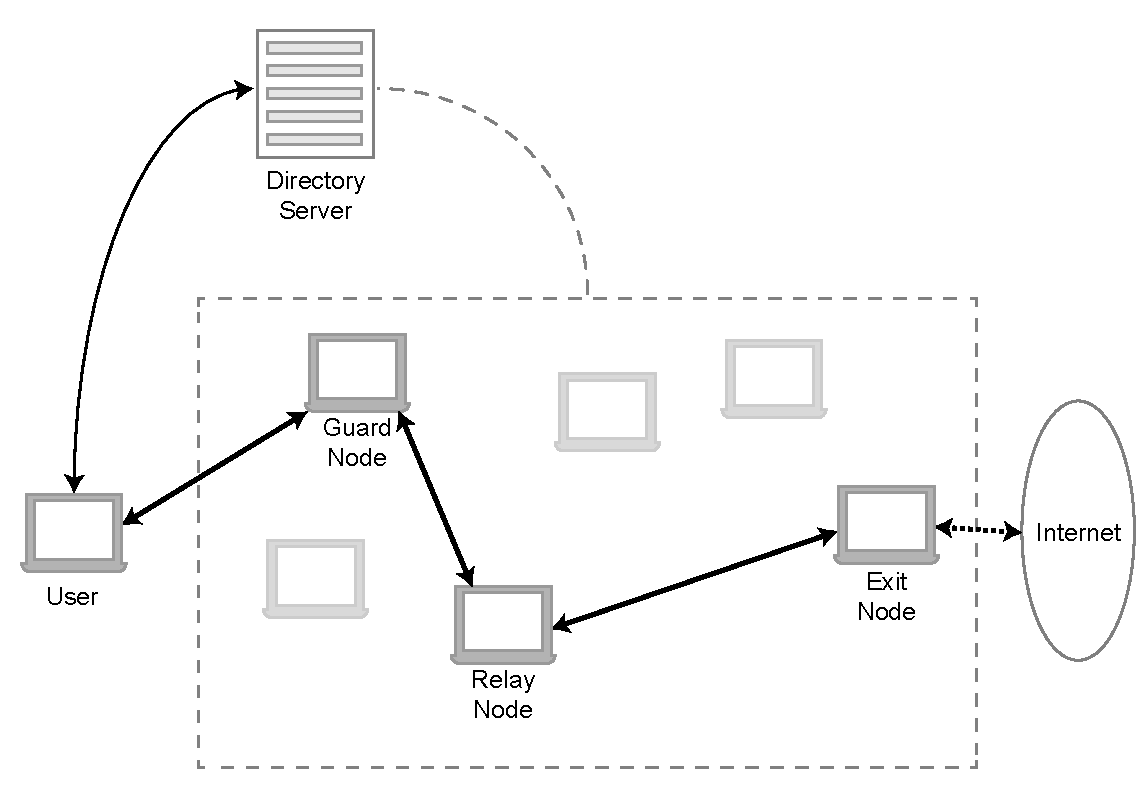
\includegraphics[width=0.8\textwidth]{graphics/tor.pdf}
		\caption{The components of the Tor network. After downloading the node list from the Directory Server, the user creates a circuit through a guard node, a relay node and an exit node. This circuit is used to communicate (anonymously) with the internet.}
		\label{fig:tor_layout}
	\end{figure*}
	
	There are several drawbacks to the current implementation of Tor. Centralized components, such as the directory server, act as a bottleneck and limit the number of possible users [CITE!!! Onze paper!]. Since anonymity in a network such as Tor is directly linked to the number of active users this is an alarming situation.
	
	The Parallel and Distributed Systems group at Delft University of Technology has implemented a Tor-like protocol in the Python programming language. This protocol is currently used in a beta version of Tribler. In contrast to Tor, it does not  use centralized components and is therefor a very scalable and secure way of communicating anonymously.

\section{Tribler}
Hier komt wat over Tribler

\subsection{What is Tribler? (Rolf)}

\subsection{M2Crypto (Martijn)}

\subsection{Tribler Mobile}

\subsection{Dispersy (Laurens)}
Dispersy [CITE NAAR DISPERY PAPER] is a fully decentralized system for data bundle synchronization used by Tribler. The system is designed in such a way that it is capable of running in a challenged network environment. Such an environment is often characterized by:
\begin{itemize}
\item Nodes randomly joining and leaving
\item Delays in the network
\item Nodes having different networking speeds (Edge, 3G, WiFi).
\item Nodes often being behind routers with Natwork Address Translating (NAT) firewalls.
\end{itemize}

All communication done by Dispersy uses UDP, because up to 64\% of the Internet is behind a NAT, they can use UDP firewall-NAT puncturing mechanisms.\\

In Dispersy, each node has a candidate list. A candidate list is a list of active connections within the node's overlay. A Dispersy node synchronizes in five steps:

\begin{enumerate}
\item First it selects a note from its candidate list.
\item It then selects a range of bundles to synchronize.
\item The node creates a Bloomfilter by hashing the selected bundles.
\item Then the node sends the created Bloomfilter to the selected node.
\item Finally, it pauses for a fixed interval to go back to step 1.
\end{enumerate}

The candidate list is divided into three sections: trusted nodes, nodes that have been successfully contacted in the past and nodes that have been connected in the past either trough an introduction-request or nodes that have been introduced.\\

A Bloomfilter use a hash area consisting of N bits, initially all set to 0. For each item that needs to be stored in the Bloomfilter, K distinct addresses are generated using a hash of the item. The bits addressed in the Bloomfilter are then set to 1. To check if an item is part of a Bloomfilter, one only has to generate the hash of that item and check if the addresses that are generated by the hash are 1 in the Bloomfilter.\\

After benchmarking Dispery against Cassandra (the database system used by Facebook), they came to the conclusion that Dispersy performs better than Cassandra. By using Bloomfilters, Dispersy can scale to over 100,000 bundles to synchronize.


\subsection{Anonymous tunnels (Martijn)}

\section{Tribler on Android (Laurens)}
Hier komt een stukje over waarom we Tribler op Android willen hebben.

\section{Python for Android (Rolf)}
Hier komt een stukje over wat Python for Android precies is, wat het doet en hoe we het kunnen gebruiken.

\section{The Global Square (Martijn)}

\subsection{What is The Global Square}

\subsection{Their contribution to Tribler}
Hier wat over de libraries die ze hebben gecompileerd voor Android

\subsection{Our project (Martijn)}
Hier wat over ons project

\end{document}
